\documentclass[10pt]{article}
\usepackage[letterpaper,text={6.5in,8.7in},centering]{geometry}
\usepackage{amssymb,amsmath,times,url,subfigure,graphicx,theorem,alltt}
%\usepackage[pdftex,urlcolor=blue,pdfpagemode=none,pdfstartview=FitH]{hyperref}

%% url smaller font.
\makeatletter
\def\url@leostyle{%
  \@ifundefined{selectfont}{\def\UrlFont{\sf}}{\def\UrlFont{\small\ttfamily}}}
\makeatother
\urlstyle{leo}

%\usepackage[all,import]{xy}

\newcommand{\norm}[1]{\ensuremath{\left\| #1 \right\|}}
\newcommand{\abs}[1]{\ensuremath{\left| #1 \right|}}
\newcommand{\bracket}[1]{\ensuremath{\left[ #1 \right]}}
\newcommand{\braces}[1]{\ensuremath{\left\{ #1 \right\}}}
\newcommand{\parenth}[1]{\ensuremath{\left( #1 \right)}}
\newcommand{\ip}[1]{\ensuremath{\langle #1 \rangle}}
\newcommand{\refeqn}[1]{(\ref{eqn:#1})}
\newcommand{\reffig}[1]{Fig. \ref{fig:#1}}
\newcommand{\tr}[1]{\mbox{tr}\ensuremath{\negthickspace\bracket{#1}}}
\newcommand{\deriv}[2]{\ensuremath{\frac{\partial #1}{\partial #2}}}
\newcommand{\SO}{\ensuremath{\mathrm{SO(3)}}}
\newcommand{\T}{\ensuremath{\mathrm{T}}}
\newcommand{\so}{\ensuremath{\mathfrak{so}(3)}}
\newcommand{\SE}{\ensuremath{\mathrm{SE(3)}}}
\newcommand{\se}{\ensuremath{\mathfrak{se}(3)}}
\renewcommand{\Re}{\ensuremath{\mathbb{R}}}
\renewcommand{\S}{\ensuremath{\mathbb{S}}}
\newcommand{\aSE}[2]{\ensuremath{\begin{bmatrix}#1&#2\\0&1\end{bmatrix}}}
\newcommand{\ase}[2]{\ensuremath{\begin{bmatrix}#1&#2\\0&0\end{bmatrix}}}
\newcommand{\D}{\ensuremath{\mathbf{D}}}
\newcommand{\pair}[1]{\ensuremath{\left\langle #1 \right\rangle}}
\newcommand{\met}[1]{\ensuremath{\langle\!\langle #1 \rangle\!\rangle}}
\newcommand{\Ad}{\ensuremath{\mathrm{Ad}}}
\newcommand{\ad}{\ensuremath{\mathrm{ad}}}
\newcommand{\g}{\ensuremath{\mathfrak{g}}}

\renewcommand{\baselinestretch}{1.2}
\date{}

\renewcommand{\thesubsection}{\arabic{subsection}. }
\renewcommand{\thesubsubsection}{\arabic{subsection}.\arabic{subsubsection} }

\theoremstyle{plain}\theorembodyfont{\normalfont}
\newtheorem{prob}{Problem}[section]
%\renewcommand{\theprob}{\arabic{section}.\arabic{prob}}
\renewcommand{\theprob}{\arabic{prob}}

\newenvironment{subprob}%
{\renewcommand{\theenumi}{\alph{enumi}}\renewcommand{\labelenumi}{(\theenumi)}\begin{enumerate}}%
{\end{enumerate}}%

\newenvironment{matlab}
{\begin{alltt}\small\renewcommand{\baselinestretch}{1.2}\selectfont}%
{\end{alltt}}


\begin{document}

\pagestyle{empty}
\section*{MAE3145: Solution for Homework 4}
%\vspace*{-0.4cm}
%\noindent{Due date: October 17, 2012}%\\%\vspace*{0.5cm}


%\begin{prob}
%Consider Asteroid 5 discussed at Question 3 of HW\#2. Its specific energy and specific angular momentum are given by $\mathcal{E}=10\,\mathrm{km^2/s^2}$, and $h=8\times 10^4\,\mathrm{km^2/s}$. We want to determine the time after periapsis passage $t$ when the true anomaly is $\theta=100^\circ$.
%\begin{subprob}
%\item Compute the semi-major axis $a$, and the eccentricity $e$.
%
%\textbf{Sol:} Since $\mathcal{E}>0$, it is a hyperbolic orbit. We have
%\begin{align*}
%a = \frac{\mu}{2\mathcal{E}} = 19930\,\mathrm{km},\quad 
%e = \sqrt{2\mathcal{E} \frac{h^2}{\mu^2} +1} = 1.3427.
%\end{align*}
%
%\item Compute the maximum true anomaly $\theta_\infty$. Is $\theta < \theta_\infty$?
%
%\textbf{Sol:} The maximum true anomaly is given by $\theta_\infty=\cos^{-1}{1/e} = 2.4101\,\mathrm{rad} = 138.09^\circ$. We have $\theta = 100^\circ < \theta_\infty$.
%
%\item Compute the hyperbolic eccentric anomaly $F$, and the hyperbolic mean anomaly $M_h$.
%
%\textbf{Sol:} The hyperbolic eccentric anomaly and the hyperbolic mean anomaly are given by
%\begin{align*}
%F = 2\tanh^{-1}\parenth{\sqrt{\frac{e-1}{e+1}} \tan\frac{\theta}{2}}=0.9855\,\mathrm{rad},\quad M_h = e\sinh F-F= 0.5638\,\mathrm{rad}.
%\end{align*}
%
%\item Show that the time after the periapsis passage is given by $t=0.6979\,\mathrm{hrs}$.
%\begin{align*}
%t = M_h \Big/ \parenth{\frac{\mu^2}{h^3} (e^2-1)^{3/2}}=2.5124\times 10^3\,\mathrm{sec} = 0.6979\,\mathrm{hrs}.
%\end{align*}
%
%\end{subprob}
%\end{prob}
%
%\begin{prob}
%An Earth-orbiting satellite has a period of $T=15.743$ hours and a periapsis radius $r_p=12756\,\mathrm{km}$. We want to determine the location of this satellite at time $t=1$ hour after periapsis passage.
%\begin{subprob}
%\item Compute the semi-major axis $a$, and the eccentricity $e$.
%
%\textbf{Sol:} Since $T = \frac{2\pi}{\sqrt{\mu}} a^{3/2}$ and $r_p = a(1-e)$, we have
%\begin{align*}
%a = \parenth{T\frac{\sqrt{\mu}}{2\pi}}^{2/3} = 31890\,\mathrm{km},\quad e=1-\frac{r_p}{a}=0.6.
%\end{align*}
%
%\item Compute the mean anomaly $M_e$.
%
%\textbf{Sol:} We have $M_e = 2\pi t/T = 0.3991\,\mathrm{rad}$. 
%
%\item Write a Matlab program to compute the eccentric anomaly $E$.
%
%\begin{matlab}
%clear all;
%close all;
%
%T=15.743*3600;
%rp=12756;
%
%mu=398600;
%a=(T*sqrt(mu)/2/pi)^(2/3);
%e=1-rp/a;
%t=1*3600;
%Me=2*pi/T*t;
%
%E=Me;
%errE=1;
%while errE > 1e-15
%    f=(E-e*sin(E)-Me);
%    fp=1-e*cos(E);
%    Enew=E-f/fp;
%    errE=norm(Enew-E);
%    E=Enew;
%end
%
%theta=2*atan(sqrt((1+e)/(1-e))*tan(E/2));
%disp(theta*180/pi);
%\end{matlab}
%\item Show that the true anomaly is given by $\theta=84.2850^\circ$.
%\textbf{Sol:} The above code returns $E=0.8498\,\mathrm{rad}$. The true anomaly is given by
%\begin{align*}
%\theta = 2\tan^{-1}\parenth{\sqrt{\frac{1+e}{1-e}}\tan\frac{E}{2}}=1.4711\,\mathrm{rad} = 84.2850^\circ.
%\end{align*}
%\end{subprob}
%%(Hint: if you want to verify your code, check that your code gives $\theta=\pi$ when $t=T/2$.)
%\end{prob}

\begin{prob} We observed the position and the velocity of a spacecraft orbiting the Earth as follows:
\begin{align*}
\vec r_0 = [6000,6000,6000]\,\mathrm{km},\quad \vec v_0 = [-5,-5,0]\,\mathrm{km/s}.
\end{align*}
Assume that $\mu = 398600 \,\mathrm{km^3/s^2}$.

\begin{subprob}
\item Using the Matlab code shown in the class, find the orbital elements $(h,e,\theta,\Omega,\omega,i)$.

\textbf{Sol:} We use the Matlab function \texttt{rv2oe.m} as follows:
\begin{matlab}
r_vec=[6000 6000 6000]';
v_vec=[-5 -5 0]';
[h,e,theta,Omega,omega,i]=rv2oe(r_vec,v_vec)
\end{matlab}
These commands yield:
\begin{matlab}
h =   4.2426e+04 (km^2/s)
e =    0.8351
theta =   -2.3146 (rad)
Omega =    0.7854 (rad)
omega =    2.9301 (rad)
i =    1.5708 (rad)
\end{matlab}

\item Write a Matlab function \texttt{oe2rv.m} that computes the position and the velocity vector for  given orbital elements. 

\textbf{Sol:}
\begin{matlab}
function [r_vec, v_vec]=oe2rv(h,e,theta,Omega,omega,i) 
xhat=[1;0;0]; 
yhat=[0;1;0]; 
zhat=[0;0;1]; 
mu=398600;

Nhat=cos(Omega)*xhat+sin(Omega)*yhat;
hhat=sin(i)*sin(Omega)*xhat-sin(i)*cos(Omega)*yhat+cos(i)*zhat;
Nthat=-sin(Omega)*cos(i)*xhat+cos(Omega)*cos(i)*yhat+sin(i)*zhat;

urhat=cos(theta+omega)*Nhat+sin(theta+omega)*Nthat;
uthat=-sin(theta+omega)*Nhat+cos(theta+omega)*Nthat;

r=h^2/mu*1/(1+e*cos(theta));
E=-1/2*mu^2/h^2*(1-e^2);
v=sqrt(2*(E+mu/r));
gam=atan2(e*sin(theta),1+e*cos(theta));

r_vec=r*urhat;
v_vec=v*cos(gam)*uthat+v*sin(gam)*urhat;
\end{matlab}

%(Hint: if you want to verify your code, check that your code returns $\vec r_0,\vec v_0$ when the orbital elements are equal to your answer to (a).)

\item Evaluate the function \texttt{oe2rv.m} for varying \texttt{theta=linspace(0,2*pi,200)}. The other five orbital elements $(h,e,\Omega,\omega,i)$ are fixed at your solution of (a). Plot the position and the velocity vector in a three-dimensional space. 

\textbf{Sol:} Matlab code is given as follows. 
\begin{matlab}
[h,e,theta,Omega,omega,i]=rv2oe(r_vec,v_vec);

theta=linspace(0,2*pi,200);
for k=1:200
     [r_vec_theta(:,k),v_vec_theta(:,k)]=oe2rv(h,e,theta(k),Omega,omega,i);
end
plot3(r_vec_theta(1,:),r_vec_theta(2,:),r_vec_theta(3,:));
hold on;
plot3(r_vec(1),r_vec(2),r_vec(3),'r*');
figure;
plot3(v_vec_theta(1,:),v_vec_theta(2,:),v_vec_theta(3,:));
hold on;
plot3(v_vec(1),v_vec(2),v_vec(3),'r*');
\end{matlab}

These commands generate the following figures in the next page.

\begin{figure}
\centerline{
	\subfigure[Position $\vec r$]{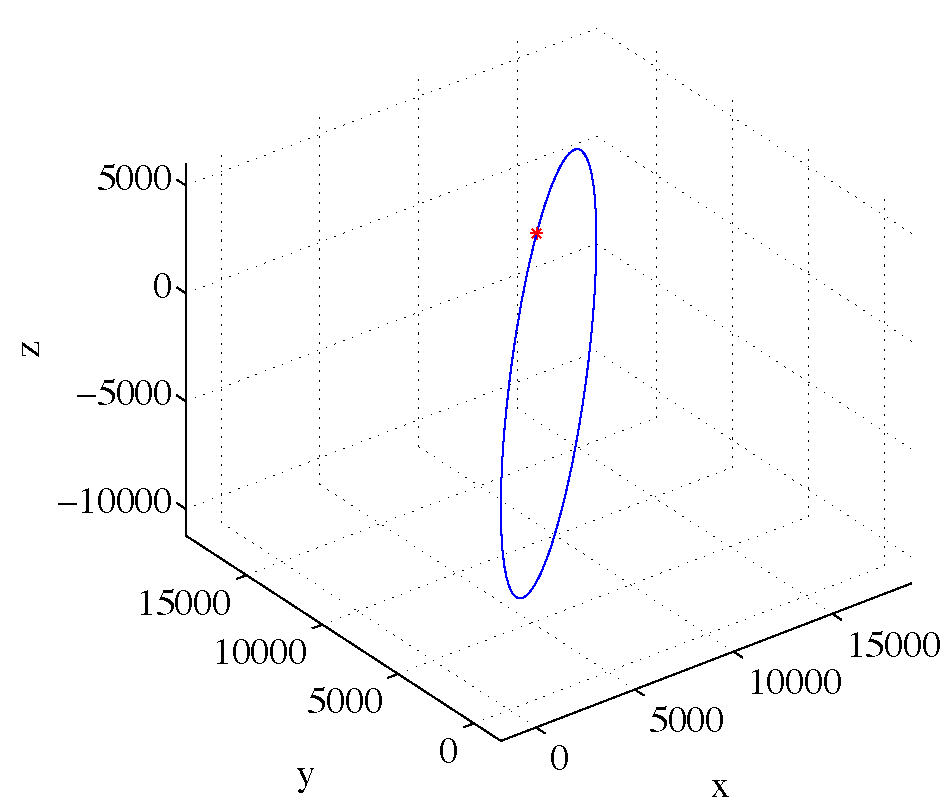
\includegraphics[height=0.4\textwidth]{prob3r.pdf}}
	\hspace*{0.1\textwidth}
	\subfigure[Velocity $\vec v$]{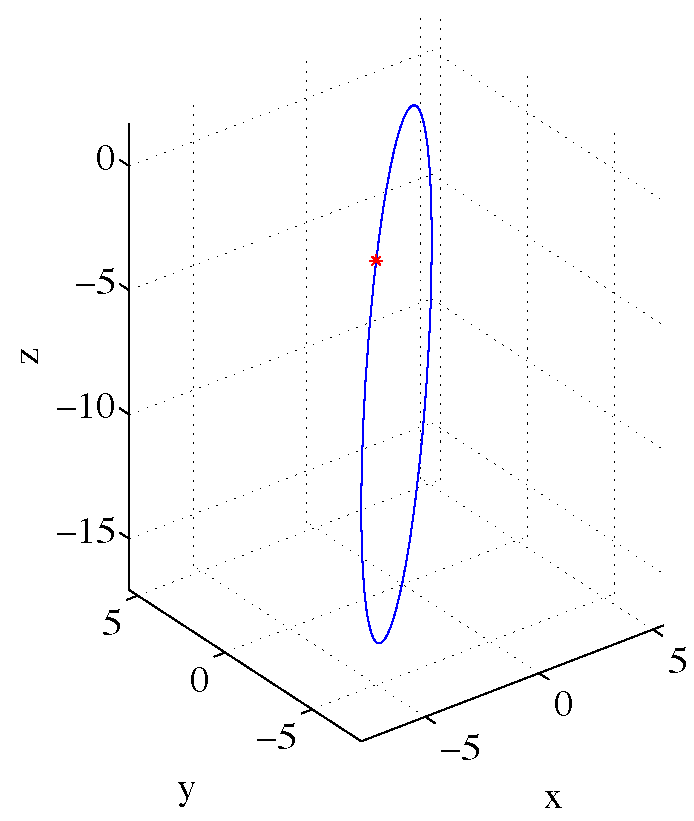
\includegraphics[height=0.4\textwidth]{prob3v.pdf}}
	}
\end{figure}

\item Check that $\vec r_0$ and $\vec v_0$ are on your curves at (c).

\textbf{Sol:} In the above figures, $\vec r_0$ and $\vec v_0$ are denoted by red stars, which are on the curves generated at (c).

\end{subprob}
\end{prob}

%\clearpage\newpage
%\begin{prob}
%In a sun-synchronous orbit, the average precession rate of $\Omega$ is the same as the orbital angular rate of the Earth around the Sun:
%\begin{align}
%\dot{\overline \Omega} = -\frac{3}{2} \frac{\sqrt{\mu} J_2 R_E^2}{(1-e^2)^2 a^{7/2}}\cos i = 2\pi \,(\mathrm{rad/year}).
%\end{align}
%Assume that $\mu = 398600 \,\mathrm{km^3/s^2}$, $R_E=6378\,\mathrm{km}$, $J_2 = 0.00108$. In this problem, we consider circular sun-synchronous orbits, i.e. $e=0$.
%\begin{subprob}
%\item Find the maximum orbital radius $a_M$ for circular sun-synchronous orbits. (Note that the orbital radius $a$ is a function of the inclination $i$.)
%\item Show that the inclination $i$ and the orbital radius $a$ of circular sun-synchronous orbits has the following relation:
%\begin{align}
%\cos i = - \parenth{\frac{a}{a_M}}^{7/2}\label{eqn:i}
%\end{align}
%\item Using \refeqn{i}, plot a curve showing the inclination as a function of the orbital radius when $R_E\leq a \leq a_M$.
%\item Find the maximum and the minimum orbit period that a circular sun-synchronous orbit can have.
%\end{subprob}
%\end{prob}

\newpage
\begin{prob} A satellite satisfies the following condition at the current time.
\begin{itemize}
\item $\vec r = [-6634.2, -1261.8, -5230.9]\,\mathrm{km}$,\quad $\vec e = [-0.40907, -0.48751, -0.63640]$
\item It is flying toward its periapsis.
\end{itemize}
\begin{subprob}
\item What is the type of orbit.

\textbf{Sol:} Since $e=\|\vec e\|= 0.9 $, it is an elliptic orbit.

\item Find the direction of the specific angular momentum $\hat h = \frac{\vec h}{h}$.

\textbf{Sol:} The vectors $\vec r$ and $\vec e$ are on the orbital plane, and the vector $\hat h$ is normal to the orbital plane. Therefore, $\hat h$ can be obtained by the cross product  of $\vec r$ and $\vec e$. Since it is flying toward its periapsis, we have $180^\circ < \theta <360^\circ$. These imply
\begin{align*}
\hat h = \frac{\vec r \times \vec e}{\|\vec r \times \vec e\|} = 
[-0.4545\,   -0.5417,\,    0.7071].
\end{align*}

\item Find the inclination $i$. %See Exercise 4.5 at page 188. Is the given solution correct?

\textbf{Sol:} The inclination is given by $i = \cos^{-1} (\hat h \cdot \hat z) = 0.7854\,\mathrm{rad}=45^\circ$.

\item Find the direction of the node vector $\hat N = \frac{\vec N}{N}$.
\textbf{Sol:} The direction of the node vector can be written as
\begin{align*}
\hat N & = \frac{\hat z \times \vec h}{\|\hat z \times \vec h\|} = 
\frac{\hat z \times \hat h}{\|\hat z \times \hat h\|} = [0.7661,   -0.6428,         0].
\end{align*}

\item[(e)-(g)]

\textbf{Sol:} Similarly, we have
\begin{align*}
\Omega & = \tan^{-1} \parenth{\frac{\hat y \cdot \hat N}{\hat x \cdot \hat N}}=-0.6981\,\mathrm{rad}=-40^\circ,\\
\omega & = \tan^{-1} \parenth{\frac{\hat h \cdot (\hat N \times \vec e)}{ (\hat N \cdot \vec e)}}=-1.5708\,\mathrm{rad}=-90^\circ,\\
\theta & = \tan^{-1} \parenth{\frac{\hat h \cdot (\vec e \times \vec r)}{ (\vec e \cdot \vec r)}}=-0.5236\,\mathrm{rad}=-30^\circ.
\end{align*}

%\item Find the longitude of the ascending node $\Omega$.
%\item Find the argument of periapsis $\omega$.
%\item Find the true anomaly $\theta$.
\end{subprob}
\end{prob}

\end{document}

